\chapter{Specifikacija programske potpore}
		
	\section{Funkcionalni zahtjevi}
			
			
			
			\noindent \textbf{Dionici:}
			
			\begin{packed_enum}
				
				\item Korisnik web aplikacije
				\item Administrator
				\item Razvojni tim
				
			\end{packed_enum}
			
			\noindent \textbf{Aktori i njihovi funkcionalni zahtjevi:}
			
			
			\begin{packed_enum}
				\item  \underbar{Neregistrirani korisnik može:}
				
				\begin{packed_enum}
					
					\item napraviti korisnički račun

					
					
				\end{packed_enum}
				
				\item  \underbar{Registrirani korisnik može:}
				
				\begin{packed_enum}
					\item prijaviti se u sustav
					\item zadati (objaviti) novi zahtjev
					\begin{packed_enum}
						\item odabrati lokaciju zahtjeva
						
					\end{packed_enum}
					\item pregledati vlastiti profil
					\begin{packed_enum}
						\item pregledati javljanja na tuđe zahtjeve
						\item upravljati korisničkim računom
						\item obrisati vlastiti korisnički račun
					\end{packed_enum}
					\item pregledati vlastite zahtjeve
					\begin{packed_enum}
						\item upravljati vlastitim zahtjevima
						\item pregledati potencijalne izvršitelje
						\begin{packed_enum}
							\item prihvatiti izvršitelja
							\item odbiti izvršitelja	
						\end{packed_enum}
					\end{packed_enum}
					\item pregledavati listu aktivnih zahtjeva
					\begin{packed_enum}
						\item filtrirati zahtjeve
						\item promijeniti lokaciju izvršavanja
						\item javiti se na zahtjev	
					\end{packed_enum}
					\item pregledati profil drugog korisnika
					\item  ocijeniti drugog korisnika
					\item izvršiti zahtjev
					\item pregledati statistiku
					\item odjaviti se iz sustava
					
				\end{packed_enum}
				\item  \underbar{Administrator}
				\begin{packed_enum}
					\item izvršavati sve mogućnosti kao registrirani korisnik
					\item dodati novog administratora	
					\item administrirati zahtjeve
					\item administrirati korisnika
				\end{packed_enum}
			\end{packed_enum}
			
			\eject 
			
			
				
			\subsection{Obrasci uporabe}
				
				
				\subsubsection{Opis obrazaca uporabe}
					\noindent \underbar{\textbf{UC1 - Registracija}}
					\begin{packed_item}
						
						\item \textbf{Glavni sudionik: }Javni korisnik
						\item  \textbf{Cilj:} Stvoriti korisnički račun u aplikaciji
						\item  \textbf{Sudionici:} Baza podataka
						\item  \textbf{Preduvjet:} -
						\item  \textbf{Opis osnovnog tijeka:}
						
						\item[] \begin{packed_enum}
							
							\item Korisnik unosi potrebne podatke
							\item Potvrda unesenih podataka
							\item Upis podataka u bazu
							\item Nakon uspješne registracije korisnik se preusmjerava na stranicu zahtjeva
						\end{packed_enum}
						
						\item  \textbf{Opis mogućih odstupanja:}
						
						\item[] \begin{packed_item}
							
							\item[1.a] Korisnik unosi već zauzeto korisničko ime i/ili e-mail ili nisu popunjena sva obavezna polja
							\item[] \begin{packed_enum}
								
								\item Prikaz odgovarajuće poruke
								\item Omogućavanje ponovnog unosa neodgovarajućih podataka
								
							\end{packed_enum}
							
							\item[4.a] Mogućnost odustajanja od registracije
							
						\end{packed_item}
					\end{packed_item}
				
					\noindent \underbar{\textbf{UC2 - Prijava u sustav}}
					\begin{packed_item}
						
						\item \textbf{Glavni sudionik: } Korisnik
						\item  \textbf{Cilj:} Prijava korisnika u sustav 
						\item  \textbf{Sudionici:} Baza podataka
						\item  \textbf{Preduvjet:} Javni korisnik ima izrađen korisnički račun u sustavu
						\item  \textbf{Opis osnovnog tijeka:}
						
						\item[] \begin{packed_enum}
							
							\item Javni korisnik odabire opciju prijave
							\item Javni korisnik upisuje korisničko ime i lozinku
							\item Korisnik potvrđuje unos
						\end{packed_enum}
						
						\item  \textbf{Opis mogućih odstupanja:}
						
						\item[] \begin{packed_item}
							
							\item[2.a] Unos pogrešnog korisničkog imena i/ili lozinke
							\item[] \begin{packed_enum}
								
								\item Javnom korisniku ispisuje se poruka o pogrešci lozinke ili korisničkog imena
								
							\end{packed_enum}
							
						\end{packed_item}
					\end{packed_item}
				
				
				
				
					\noindent \underbar{\textbf{UC3.1 - Pregled potencijalnih izvršitelja}}
					\begin{packed_item}
						
						\item \textbf{Glavni sudionik: }Korisnik autor
						\item  \textbf{Cilj:} Pregledati listu korisnika koji su se javili kao potencijalni izvršitelji
						\item  \textbf{Sudionici:}-
						\item  \textbf{Preduvjet:} Korisnik pregledava zahtjev kojem je autor
						\item  \textbf{Opis osnovnog tijeka:}
						
						
						\item[] \begin{packed_enum}
							
							\item Korisnik u prikazu zahtjeva bira opciju za prikaz potencijalnih izvršitelja
							\item Prikaz potencijalnih izvršitelja s opcijama za prihvaćanje i odbijanja
						\end{packed_enum}
						
						
					\end{packed_item}
				
				
					\noindent \underbar{\textbf{UC3.1.1 - Odbijanje javljanja na zahtjev}}
					\begin{packed_item}
						
						\item \textbf{Glavni sudionik: }Korisnik autor
						\item  \textbf{Cilj:} Odbijanje pojedinog ili više potencijalnih izvršitelja
						\item  \textbf{Sudionici:} Korisnik izvršitelj
						\item  \textbf{Preduvjet:} Postoji barem jedan potencijalni izvršitelj za zahtjev
						\item  \textbf{Opis osnovnog tijeka:}
						
						\item[] \begin{packed_enum}
							
							\item Prikaz liste potencijalnih izvršitelja
							\item Korisnik odbija pojedino javljanje na zahtjev
							\item Odbijenom korisniku šalje se obavijest o odbijanju
						\end{packed_enum}
						
					\end{packed_item}
				
				
					
					\noindent \underbar{\textbf{UC3.1.2 - Prihvaćanje javljanja na zahtjev}}
					\begin{packed_item}
						
						\item \textbf{Glavni sudionik: }Korisnik autor
						\item  \textbf{Cilj:} Prihvaćanje javljanja na zahtjev za pomoć 
						\item  \textbf{Sudionici:} Korisnik izvršitelj
						\item  \textbf{Preduvjet:} Postoji barem jedan potencijalni izvršitelj za zahtjev, Zahtjev je aktivan
						\item  \textbf{Opis osnovnog tijeka:}
						
						\item[] \begin{packed_enum}
							
							\item Prikaz liste potencijalnih izvršitelja
							\item Korisnik prihvaća pojedino javljanje na zahtjev
							\item Slanje obavijesti prihvaćenom korisniku
							\item Automatsko odbijanje ostalih potencijalnih izvršitelja
							\item Slanje obavijesti odbijenim korisnicima
							\item Automatsko dodavanje prihvaćenog korisnika kao izvršitelja zahtjeva
						\end{packed_enum}
						
					\end{packed_item}
				
					\noindent \underbar{\textbf{UC3.2 - Javljanje na zahtjev}}
					\begin{packed_item}
						
						\item \textbf{Glavni sudionik: }Korisnik
						\item  \textbf{Cilj:} Inicijalizirati komunikaciju s korisnikom autorom
						\item  \textbf{Sudionici:} Korisnik autor zahtjeva, Baza podataka
						\item  \textbf{Preduvjet:} Oglas je aktivan, korisnik nije autor zahtjeva kojeg pregledava
						\item  \textbf{Opis osnovnog tijeka:}
						
						\item[] \begin{packed_enum}
							
							\item Korisnik odabire zahtjev za pregled
							\item Korisnik odabire opciju javljanja na zahtjev
							\item Korisnik se uvodi u bazu podataka kao potencijalni izvršitelj za odabrani zahtjev
							\item Korisniku autoru dolazi obavijest o novom potencijalnom izvršitelju
						\end{packed_enum}
						
						\item  \textbf{Opis mogućih odstupanja:}
						
						\item[] \begin{packed_item}
							
							\item[1.a] Korisnik autor može biti blokiran
							\item[] \begin{packed_enum}
								
								\item Zahtjevi blokiranih korisnika ne prikazuju se na glavnoj stranici zahtjeva
								\item Zahtjevi blokiranih korisnika vidljivi na njegovom profilu ne mogu biti odabrani za izvršavanje
								
							\end{packed_enum}				
						\end{packed_item}
					\end{packed_item}
				
					\noindent \underbar{\textbf{UC3.3 - Brisanje/blokiranje zahtjeva}}
					\begin{packed_item}
						
						\item \textbf{Glavni sudionik: }Korisnik autor
						\item  \textbf{Cilj:} Mogućnost blokiranja ili brisanja zahtjeva
						\item  \textbf{Sudionici:} Baza podataka
						\item  \textbf{Preduvjet:} Korisnik pregledava vlastiti zahtjev
						\item  \textbf{Opis osnovnog tijeka:}
						
						\item[] \begin{packed_enum}
							
							\item Korisnik odabire zahtjev za pregled
							\item Korisnik odabire brisanje/blokiranje zahtjeva
							\item Unos izmjena u bazu podataka
							
						\end{packed_enum}
					
						\item  \textbf{Opis mogućih odstupanja:}
						
						\item[] \begin{packed_item}
							
							\item[2.a] Pokušaj brisanja/blokiranja zahtjeva za koje postoje aktivni izvršitelji
							\item[] \begin{packed_enum}
								
								\item Zahtjevi za koje postoje aktivni izvršitelji mogu biti samo blokirani 
								\item Svim potencijalnim ili aktivnim izvršiteljima se šalje obavijest o blokiranju zahtjeva
								
							\end{packed_enum}				
						\end{packed_item}
						
					\end{packed_item}
				
					\noindent \underbar{\textbf{UC4 - Zadavanje novog zahtjeva}}
					\begin{packed_item}
						
						\item \textbf{Glavni sudionik: }Korisnik
						\item  \textbf{Cilj:} Unijeti i opisati svoj zahtjev za pomoć
						\item  \textbf{Sudionici:} Baza podataka
						\item  \textbf{Preduvjet:} Korisnik je prijavljen
						\item  \textbf{Opis osnovnog tijeka:}
						
						\item[] \begin{packed_enum}
							
							\item Korisnik otvara komponentu za unos zahtjeva
							\item Unos opisa zahtjeva
							\item Unos vremena isteka
							\item Potvrda zahtjeva
							\item Unos zahtjeva u bazu podataka
						\end{packed_enum}
						
						\item  \textbf{Opis mogućih odstupanja:}
						
						\item[] \begin{packed_item}
							
							\item[2.a] Unos zahtjeva sa praznim opisom
							\item[] \begin{packed_enum}
								
								\item Prikaz poruke o minimalnoj duljini opisa od dva znaka
								
							\end{packed_enum}
							
						\end{packed_item}
					\end{packed_item}
				
					\noindent \underbar{\textbf{UC4.1 - Odabir lokacije zahtjeva}}
					\begin{packed_item}
						
						\item \textbf{Glavni sudionik: }Korisnik
						\item  \textbf{Cilj:} Opcionalan odabir lokacije zahtjeva
						\item  \textbf{Sudionici:} Baza podataka
						\item  \textbf{Preduvjet:} U tijeku je zadavanje novog zahtjeva
						\item  \textbf{Opis osnovnog tijeka:}
						
						\item[] \begin{packed_enum}
							
							\item Korisnik se odlučuje za postavljanje lokacije
							\item Odabir korištenja adrese korisnika ili unosa na karti
							\item Otvaranje karte za unos lokacije
							\item Potvrda lokacije
							\item Nastavak zadavanja zahtjeva
						\end{packed_enum}
						
						\item  \textbf{Opis mogućih odstupanja:}
						
						\item[] \begin{packed_item}
							
							
							\item[1.a] Korisnik se odlučuje ne unositi lokaciju
							\item[] \begin{packed_enum}
								
								\item Zahtjevi bez lokacije vode se kao virtualni i prikazuju se svim korisnicima
								\item Virtualni zahtjevi polaze od pretpostavke da je lokacija irelevantna za uspješno izvršavanje
							
								\end{packed_enum}	
							\item[3.a] Unos prazne lokacije
							\item[] \begin{packed_enum}
								\item Ukoliko se korisnik odlučio za unos lokacije putem karte, a nije to učinio kao adresa zahtjeva se vodi nulti meridijan i ekvator.
							\end{packed_enum} 						
						\end{packed_item}
					\end{packed_item}
				
				
					\noindent \underbar{\textbf{UC5 - Pregled profila}}
					\begin{packed_item}
						
						\item \textbf{Glavni sudionik: }Korisnik
						\item  \textbf{Cilj:} Pregled profila korisnika 
						\item  \textbf{Sudionici:} Baza podataka
						\item  \textbf{Preduvjet:} -
						\item  \textbf{Opis osnovnog tijeka:}
						
						\item[] \begin{packed_enum}
							
							\item Odabir korisnika za prikaz
							\item Prikaz osnovnih podataka o korisniku, njegovih zahtjeva i zahtjeva koje je on izvršio
							\item Korisnik može pregledavati zahtjeve profila
							\item Korisnik može pregledati lanac povjerenja, komentare i ocjenu profila korisnika
						\end{packed_enum}
						
					\end{packed_item}
				
					
				
					\noindent \underbar{\textbf{UC5.1 - Brisanje korisničkog računa}}
					\begin{packed_item}
						
						\item \textbf{Glavni sudionik: }Korisnik
						\item  \textbf{Cilj:} Brisanje korisničkog računa iz sustava 
						\item  \textbf{Sudionici:} Baza podataka
						\item  \textbf{Preduvjet:} -
						\item  \textbf{Opis osnovnog tijeka:}
						
						\item[] \begin{packed_enum}
							
							\item Korisnik odabire opciju brisanja računa
							\item Unos brisanja u bazu podataka
							
						\end{packed_enum}
						
					\end{packed_item}
				
					\noindent \underbar{\textbf{UC5.2 - Upravljanje korisničkim podacima}}
					\begin{packed_item}
						
						\item \textbf{Glavni sudionik: }Korisnik
						\item  \textbf{Cilj:} Izmjena korisničkih podataka 
						\item  \textbf{Sudionici:} Baza podataka
						\item  \textbf{Preduvjet:} -
						\item  \textbf{Opis osnovnog tijeka:}
						\item[] \begin{packed_enum}
							
							\item Korisnik odabire opciju izmjene korisničkih podataka
							\item Korisnik unosi nove podatke
							\item Korisnik potvrđuje novi unos
							
						\end{packed_enum}
						\item  \textbf{Opis mogućih odstupanja:}
						
					
						\item[] \begin{packed_item}
							
							\item[2.a] Unos podataka u krivom formatu ili neispunjenje obaveznih polja
							\item[] \begin{packed_enum}
								
								\item Prikaz odgovarajuće poruke
								\item Ponovna mogućnost unosa podataka
								
							\end{packed_enum}
							
						\end{packed_item}
						
					\end{packed_item}
				
				
					\noindent \underbar{\textbf{UC6 - Promjena lokacije izvršenja}}
					\begin{packed_item}
						
						\item \textbf{Glavni sudionik: }Korisnik
						\item  \textbf{Cilj:} Izmjena korisnikove lokacije
						\item  \textbf{Sudionici:} Baza podataka
						\item  \textbf{Preduvjet:} -
						\item  \textbf{Opis osnovnog tijeka:}
						
						\item[] \begin{packed_enum}
							
							\item Korisnik odabire izmjenu lokacije
							\item Korisnik unosi novu lokaciju u tekstualnom obliku ili odabirom na karti
							\item Nova lokacija pohranjuje se u bazu
							\item Prikaz zahtjeva u odnosu na novu lokaciju
						\end{packed_enum}
						
						\item  \textbf{Opis mogućih odstupanja:}
						
						\item[] \begin{packed_item}
							
							\item[3.a] Unos nevaljane lokacije
							\item[] \begin{packed_enum}
								
								\item Unos lokacije u bazu se stornira
								\item Korisniku se prikazuje odgovarajuća poruka
								
							\end{packed_enum}

						\end{packed_item}
					\end{packed_item}
				
					\noindent \underbar{\textbf{UC7 - Izvršavanje zahtjeva}}
					\begin{packed_item}
						
						\item \textbf{Glavni sudionik: }Korisnik
						\item  \textbf{Cilj:} Označavanje zahtjeva izvršenim 
						\item  \textbf{Sudionici:} Baza podataka
						\item  \textbf{Preduvjet:} Korisnik je postavljen kao autor zahtjeva
						\item  \textbf{Opis osnovnog tijeka:}
						
						\item[] \begin{packed_enum}
							
							\item Korisnik odabire zahtjev za pregled
							\item Korisnik označuje zahtjev izvršenim
							\item Korisniku izvršitelju šalje se obavijest o izvršenju
							\item Inicira se ocjenjivanje korisnika
							
						\end{packed_enum}
					
			
						\item  \textbf{Opis mogućih odstupanja:}
							
							\item[] \begin{packed_item}
															
							\item[1.a] Zahtjev je istekao prije nego što je korisnik potvrdio izvršenje
							\item[] \begin{packed_enum}
								
								\item Zahtjevi za koje je korisnik odabran kao izvršitelj prikazuju se unatoč istjecanju i mogu se odabrati za izvršavanje
								
							\end{packed_enum}
							\item[1.b] Zahtjev za koji je korisnik odabran kao izvršitelj je blokiran
							\item[] \begin{packed_enum}
								
								\item Blokirani zahtjevi se ne mogu izvršavati i ne prikazuju se među korisnikovim zahtjevima za izvršavanje
								
									\end{packed_enum}
							

						\end{packed_item}
				\end{packed_item}
				
					\noindent \underbar{\textbf{UC8 - Ocjenjivanje korisnika}}
					\begin{packed_item}
						
						\item \textbf{Glavni sudionik: }Korisnik
						\item  \textbf{Cilj:} Ocjena korisnika i/ili ocjena izvršenja zahtjeva uz popratni komentar 
						\item  \textbf{Sudionici:} Baza podataka
						\item  \textbf{Preduvjet:} -
						\item  \textbf{Opis osnovnog tijeka:}
						
						\item[] \begin{packed_enum}
							
							\item Korisnik inicira ocjenjivanje na profilu drugog korisnika ili se ocjenjivanje pokreće nakon izvršenja zahtjeva
							\item Korisnik izabire ocjenu od 1 do 5
							\item Korisnik opcionalno unosi komentar
							\item Korisnik potvrđuje svoj odabir
							\item Ocjena i komentar se unose u bazu podataka
						\end{packed_enum}
						
						\item  \textbf{Opis mogućih odstupanja:}
						
						\item[] \begin{packed_item}
							
							\item[2.a] Ocjena se može, ali ne mora odnositi na izvršavanje specifičnog zahtjeva
							\item[] \begin{packed_enum}
								
								\item Ukoliko se ocjena odnosi na izvršavanje zahtjeva, u bazu se upisuje o kojem se zahtjevu radi
								
							\end{packed_enum}
							
						\end{packed_item}
					\end{packed_item}
				
				
					\noindent \underbar{\textbf{UC9 - Pregled statistike}}
					\begin{packed_item}
						
						\item \textbf{Glavni sudionik: }Korisnik
						\item  \textbf{Cilj:} Prikaz statistika o korisnicima 
						\item  \textbf{Sudionici:} Baza podataka
						\item  \textbf{Preduvjet:} -
						\item  \textbf{Opis osnovnog tijeka:}
						
						\item[] \begin{packed_enum}
							
							\item Korisnik odabire opciju prikaza statistike
							\item Prikaz statistike u aplikaciji
							\item Povratak na prethodnu stranicu
							
						\end{packed_enum}
						
					\end{packed_item}
				
				
					\noindent \underbar{\textbf{UC10 - Administriranje zahtjeva}}
					\begin{packed_item}
						
						\item \textbf{Glavni sudionik: }Administrator
						\item  \textbf{Cilj:} Brisanje neprihvatljivih zahtjeva 
						\item  \textbf{Sudionici:} Baza podataka
						\item  \textbf{Preduvjet:} -
						\item  \textbf{Opis osnovnog tijeka:}
						
						\item[] \begin{packed_enum}
							
							\item Administrator odabire opciju brisanja zahtjeva
							\item Administrator potvrđuje odabir
							\item Autoru zahtjeva dolazi obavijest o brisanju zahtjeva
							\item Potencijalnim izvršiteljima se šalje obavijest o brisanju zahtjeva
						\end{packed_enum}
						
						\item  \textbf{Opis mogućih odstupanja:}
						
						\item[] \begin{packed_item}
							
							\item[2.a] Javljanje na zahtjev je već prihvaćeno i izvršitelj je postavljen
							\item[] \begin{packed_enum}
								
								\item Izvršitelj dobiva obavijest o brisanju zahtjeva
								
							\end{packed_enum}
							
						\end{packed_item}
					\end{packed_item}	
				
				
					\noindent \underbar{\textbf{UC11 - Administriranje korisnika}}
					\begin{packed_item}
						
						\item \textbf{Glavni sudionik: }Administrator
						\item  \textbf{Cilj:} Upravljanje korisnicima 
						\item  \textbf{Sudionici:} Korisnici, Baza podataka
						\item  \textbf{Preduvjet:} -
						\item  \textbf{Opis osnovnog tijeka:}
						
						\item[] \begin{packed_enum}
							
							\item Na profilu korisnika administrator odabire opciju administriranja korisnika
							\item Administrator bira opciju privremenog ili trajnog blokiranja korisnika
							\item Administrator potvrđuje odabir
							\item Unos blokiranja u bazu podataka
							\item Svi aktivni zahtjevi blokiranog korisnika za koje nije još odabran izvršitelj se brišu
						\end{packed_enum}
					
						\item  \textbf{Opis mogućih odstupanja:}
						
						\item[] \begin{packed_item}
							
							\item[1.a] Korisnik je već privremeno blokiran
							\item[] \begin{packed_enum}
								
								\item Administrator može odblokirati privremeno blokiranog korisnika
								
							\end{packed_enum}
						  
							\item[1.b] Korisnik je već trajno blokiran
							\item[] \begin{packed_enum}
								
								\item Administrator ne može odblokirati trajno blokiranog korisnika
								
							\end{packed_enum}
					
					
						
					\end{packed_item}
				\end{packed_item}
				
				
					\noindent \underbar{\textbf{UC12 - Dodavanje novog administratora}}
					\begin{packed_item}
						
						\item \textbf{Glavni sudionik: }Administrator
						\item  \textbf{Cilj:} Postaviti nekog korisnika kao administratora 
						\item  \textbf{Sudionici:} Baza podataka
						\item  \textbf{Preduvjet:} -
						\item  \textbf{Opis osnovnog tijeka:}
						
						\item[] \begin{packed_enum}
							
							\item Administrator na profilu korisnika odabire opciju postavljanja administratorskih ovlasti
							\item Administrator potvrđuje odabir
							
						\end{packed_enum}
						
						\item  \textbf{Opis mogućih odstupanja:}
						
						\item[] \begin{packed_item}
							
							\item[1.a] Pregledavanje profila korisnika koji već ima dodijeljene administratorske ovlasti
							\item[] \begin{packed_enum}
								
								\item Administratoru se ne omogućava ponovo postavljanje ovlasti
								
							\end{packed_enum}
							
						\end{packed_item}
					\end{packed_item}
				
					\noindent \underbar{\textbf{UC13 - Odjava}}
					\begin{packed_item}
						
						\item \textbf{Glavni sudionik: }Korisnik
						\item  \textbf{Cilj:} Odjava iz sustava 
						\item  \textbf{Sudionici:} -
						\item  \textbf{Preduvjet:} Korisnik je prijavljen u sustav
						\item  \textbf{Opis osnovnog tijeka:}
						
						\item[] \begin{packed_enum}
							
							\item Korisnik odabire opciju odjave
							\item Korisnik se preusmjerava na stranicu za prijavu
						\end{packed_enum}
						
					\end{packed_item}
					
					\newpage
			
					
					
				\subsubsection{Dijagrami obrazaca uporabe}
					
					\begin{figure}[H]
					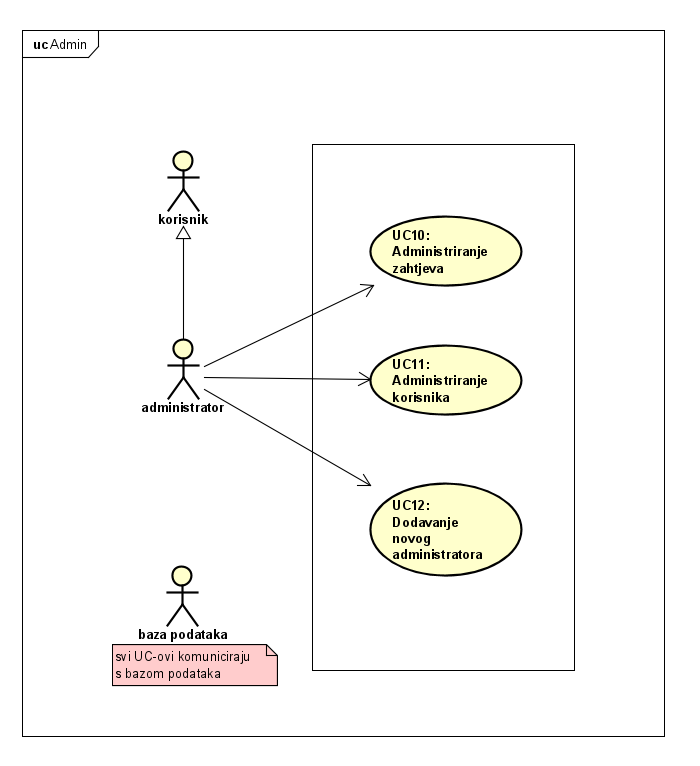
\includegraphics[scale=1.0]{slike/admin.png} %veličina slike u odnosu na originalnu datoteku i pozicija slike
					\centering
					\caption{Admin}
				\end{figure}
				
				
					\begin{figure}[H]
					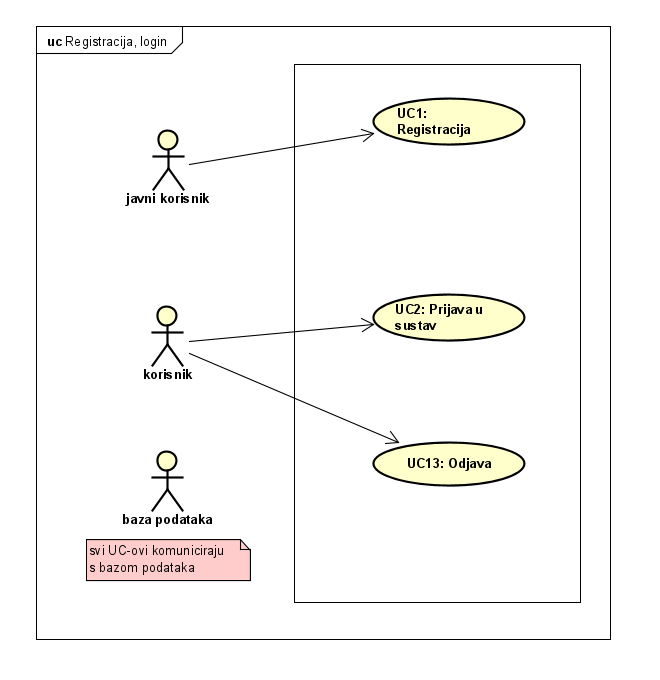
\includegraphics[scale=1.0]{slike/reg-log.png} %veličina slike u odnosu na originalnu datoteku i pozicija slike
					\centering
					\caption{Registracija, login}
				\end{figure}
				
				
					\begin{figure}[H]
					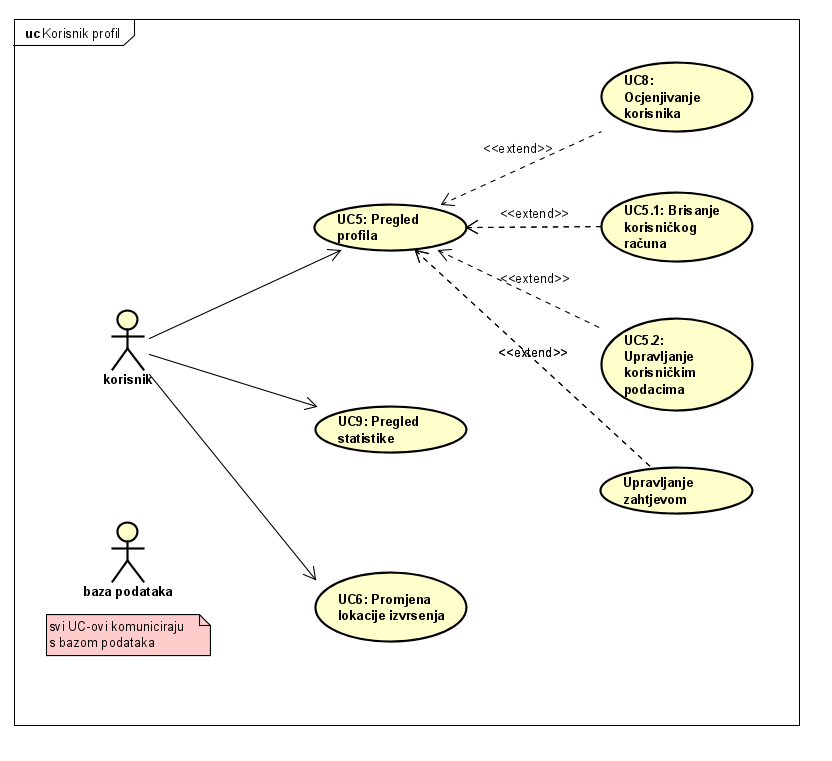
\includegraphics[scale=0.9]{slike/korisnik-profil.png} %veličina slike u odnosu na originalnu datoteku i pozicija slike
					\centering
					\caption{Korisnik i profil}
				\end{figure}
				
				
					\begin{figure}[H]
					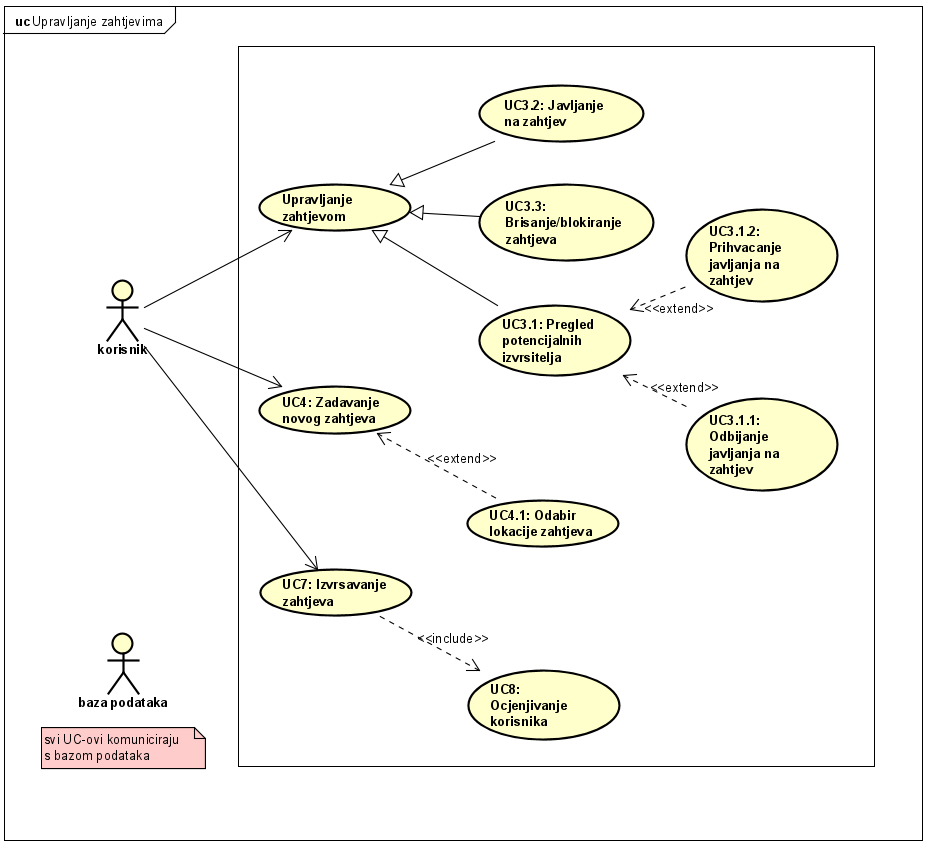
\includegraphics[scale=0.9]{slike/upravljanje-zahtjevima.png} %veličina slike u odnosu na originalnu datoteku i pozicija slike
					\centering
					\caption{Upravljanje zahtjevima}
				\end{figure}
				\newpage
				
				
				\eject		
				
			\subsection{Sekvencijski dijagrami}
				
				\noindent \large {\textbf{Novi zahtjev}}
				\newline
				\noindent \normalsize Pri postavljanju novog zahtjeva, korisnik odabire opciju za dodavanje novog zahtjeva te mu poslužitelj šalje formu novog zahtjeva. Nakon toga, korisnik popunjava formu te ga sustav traži da popravi unos dok god su neka polja krivo popunjena. Nakon uspješne popune svih polja u formi, događa se evidentiranje zahtjeva u bazi, te se nakon toga zahtjev može prikazivati drugim korisnicima aplikacije. 
				   
				
				\begin{figure}[H]
					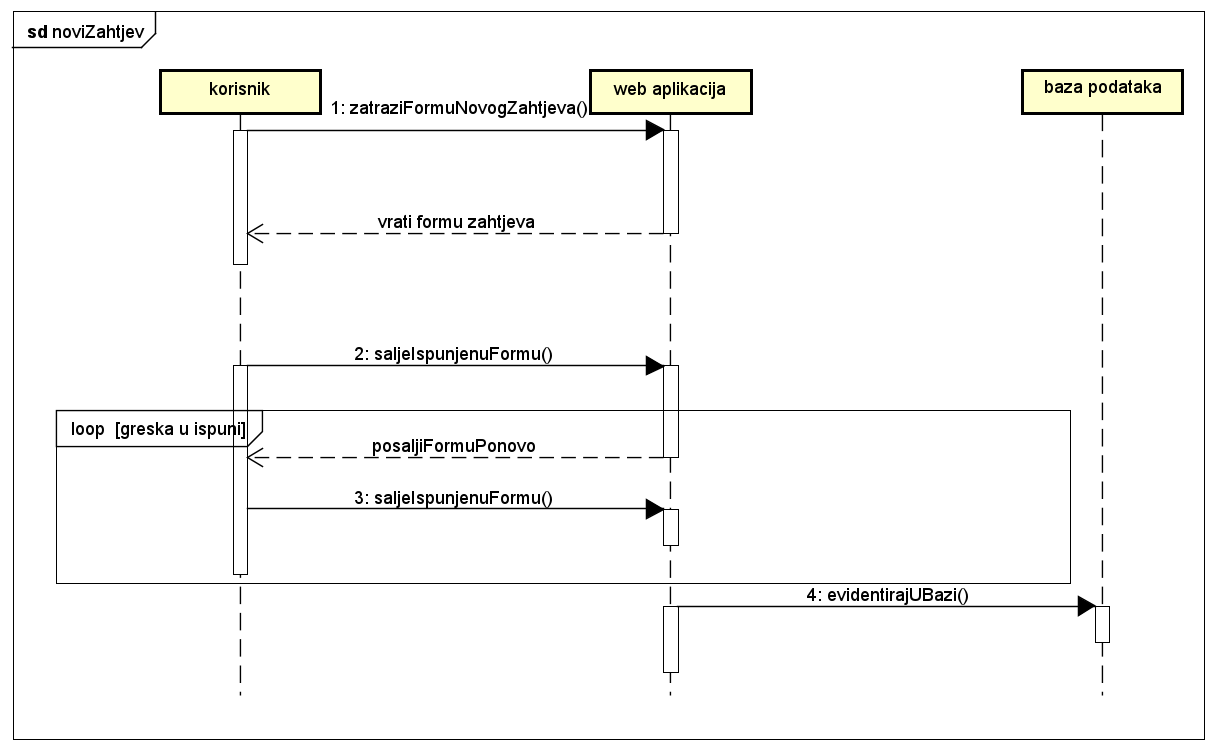
\includegraphics[scale=0.5]{slike/novi-zahtjev.png} %veličina slike u odnosu na originalnu datoteku i pozicija slike
					\centering
					\caption{Novi zahtjev}
				\end{figure}
				\newpage
				
				\noindent \large {\textbf{Pregled zahtjeva, javljanje na zahtjev}}
				\newline
				\noindent \normalsize Korisnik pri uobičajenom korištenju aplikacije može pregledavati listu dostupnih zahtjeva. Korisnik tada odabire opciju prikaza zahtjeva, a poslužitelj od baze podataka traži odgovarajuće zahtjeve obzirom na kriterije filtriranja zahtjeva za prikaz. U slučaju da postoje aktivni zahtjevi sa odgovarajućim uvjetima korisnik ima mogućnost javiti se na zahtjev tako što odabere tu opciju u aplikaciji, a poslužitelj to evidentira u bazi. Nakon što se javio na zahtjev, autor zahtjeva može vidjeti kontakte potencijalnih izvršitelja i kontaktirati ih. U slučaju da nema aktivnih zahtjeva korisniku se u aplikaciji ispisuje odgovarajuća poruka te nema daljnjih mogućnosti za javljanje na zahtjev. 
				   
				
				\begin{figure}[H]
					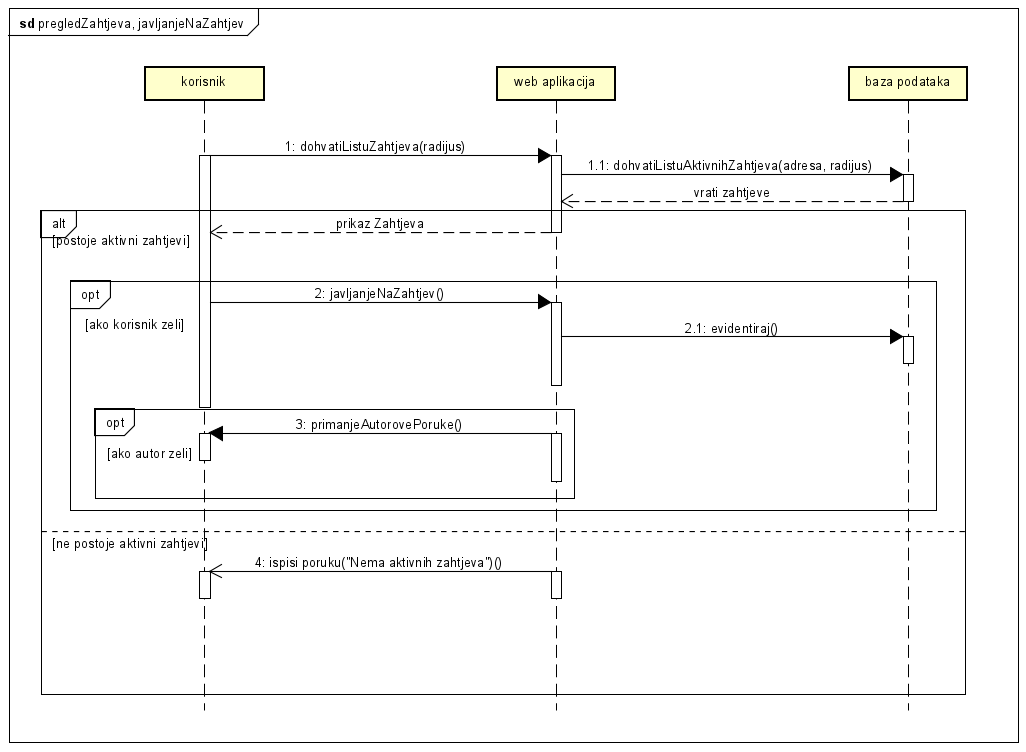
\includegraphics[scale=0.7]{slike/pregled-zahtjeva.png} %veličina slike u odnosu na originalnu datoteku i pozicija slike
					\centering
					\caption{Pregled zahtjeva, javljanje na zahtjev}
				\end{figure}
				\newpage
								
				\noindent \large {\textbf{Biranje izvršitelja}}
				\newline
				\noindent \normalsize Isprva korisnik šalje zahtjev za prikazivanjem njegovih aktivnih zahtjeva, poslužitelj ih pronalazi u bazi i prosljeđuje korisniku. Ako korisnik želi vidjeti neki pojedini zahtjev detaljnije, odabire taj zahtjev te mu se u slučaju da postoje ljudi koji su se javili na zahtjev nude opcije odbijanja i prihvaćanja pojedinog izvršitelja te može isto tako odgoditi odluko oko biranja izvršitelja i vratiti se na prikaz svih njegovih aktivnih zahtjeva. 
				   
				
				\begin{figure}[H]
					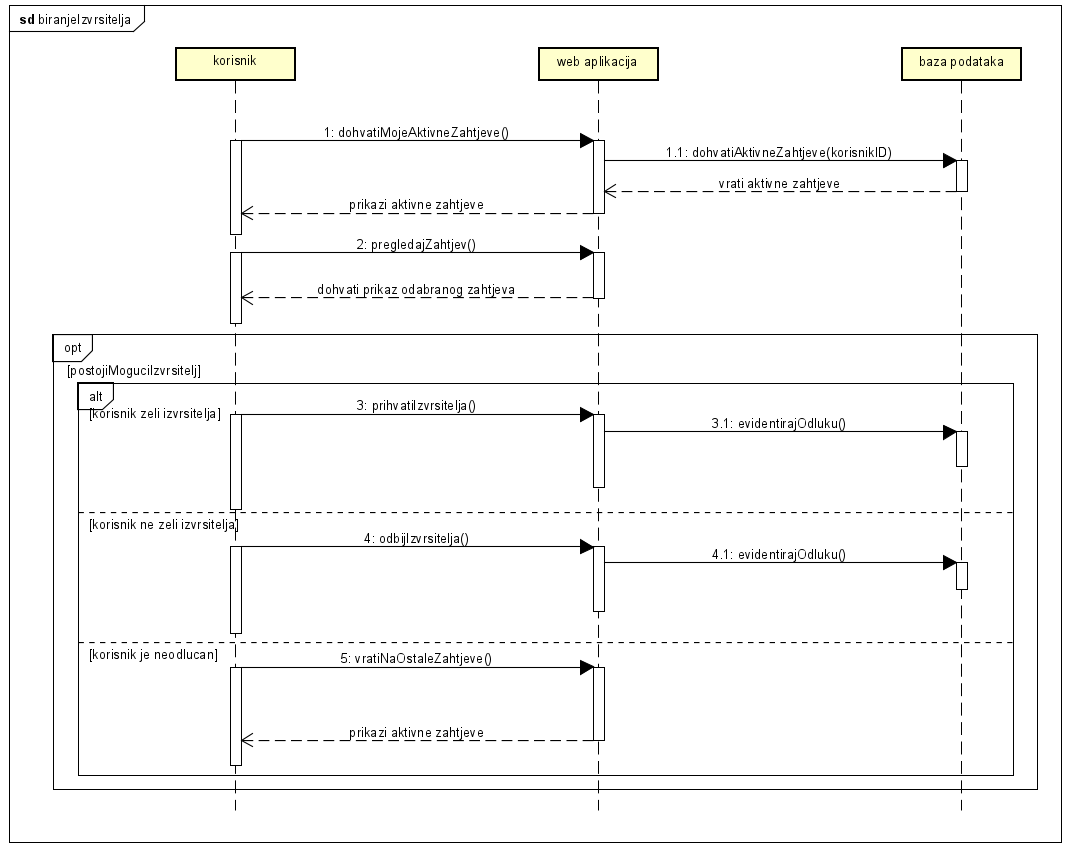
\includegraphics[scale=0.6]{slike/biranje-izvrsitelja.png} %veličina slike u odnosu na originalnu datoteku i pozicija slike
					\centering
					\caption{Biranje izvršitelja}
				\end{figure}
				\newpage
				
				\noindent \large {\textbf{Izvršavanje viša razina}}
				\newline
				\noindent \normalsize Izvršavanje kreće tako da sustav šalje kontakte izvršitelju i autoru. Nakon izvršavanja autor označava da je zahtjev izvršen, čime se omogućava ocjenjivanje. Ocjenjivanje uključuje odabir ocjene od 1 do 5 te opcionalan unos komentara.
				   
							
				\begin{figure}[H]
					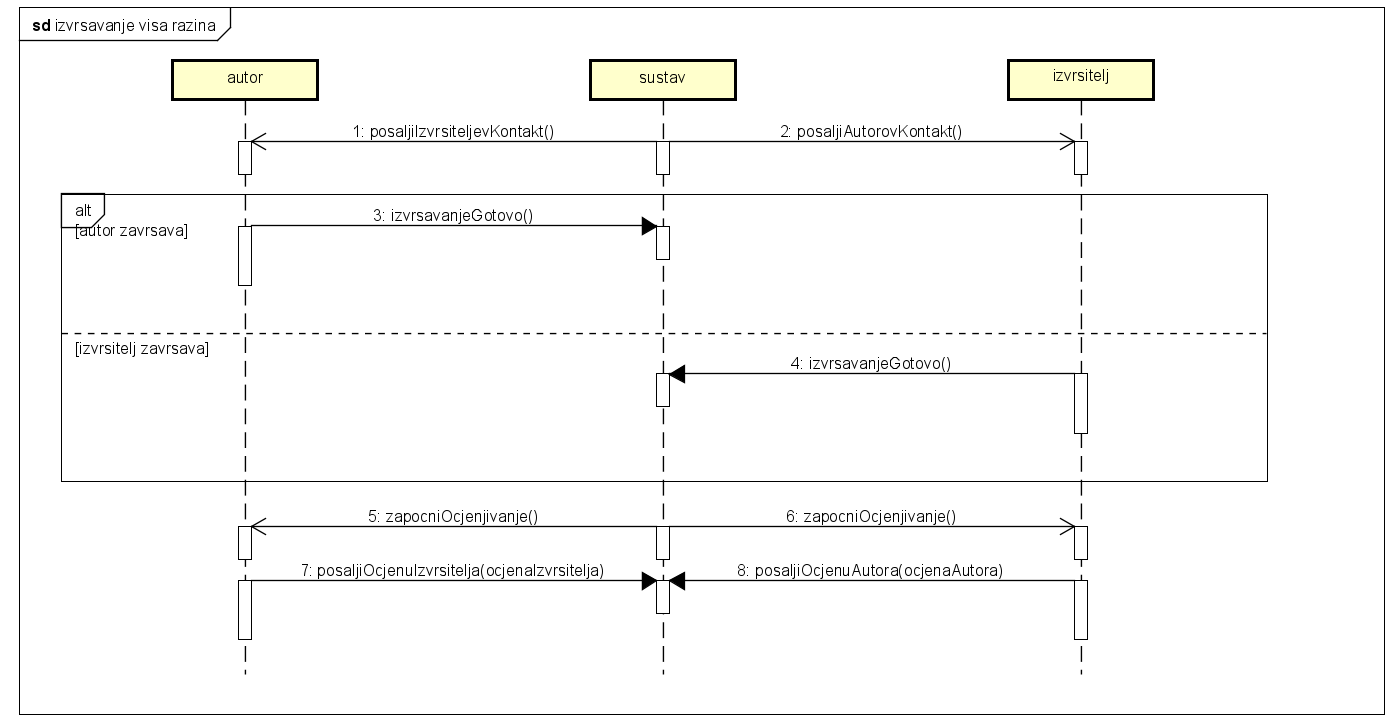
\includegraphics[scale=0.65]{slike/izvrsavanje-visa-razina.png} %veličina slike u odnosu na originalnu datoteku i pozicija slike
					\centering
					\caption{Izvršavanje viša razina}
				\end{figure}
				
				\newpage
				\eject
	
		\section{Ostali zahtjevi}
		
		\begin{itemize}
			\item Aplikacija treba biti izvedena kao web aplikacija prilagođena mobilnom uređaju.
			\item Sustav mora podržavati rad više korisnika u stvarnom vremenu.
			\item Procesiranje bilo kakve korisničke interakcije sa sustavom ne bi trebalo trajati duže od par sekundi.
			\item Administratori su dodijeljeni po geografskim lokacijama.
			\item Sustav mora podržavati hrvatske dijakritičke znakove.
			\item Informacije o zahtjevima moraju biti redovno ažurirane.
			\item Korisničko sučelje treba biti jednostavno za korištenje.
		\end{itemize}
			 
			 
			 
	